\subsubsection{\idx{Pitagora}}

\zadatak Odredi $x$ sa slike.
$$
\slika{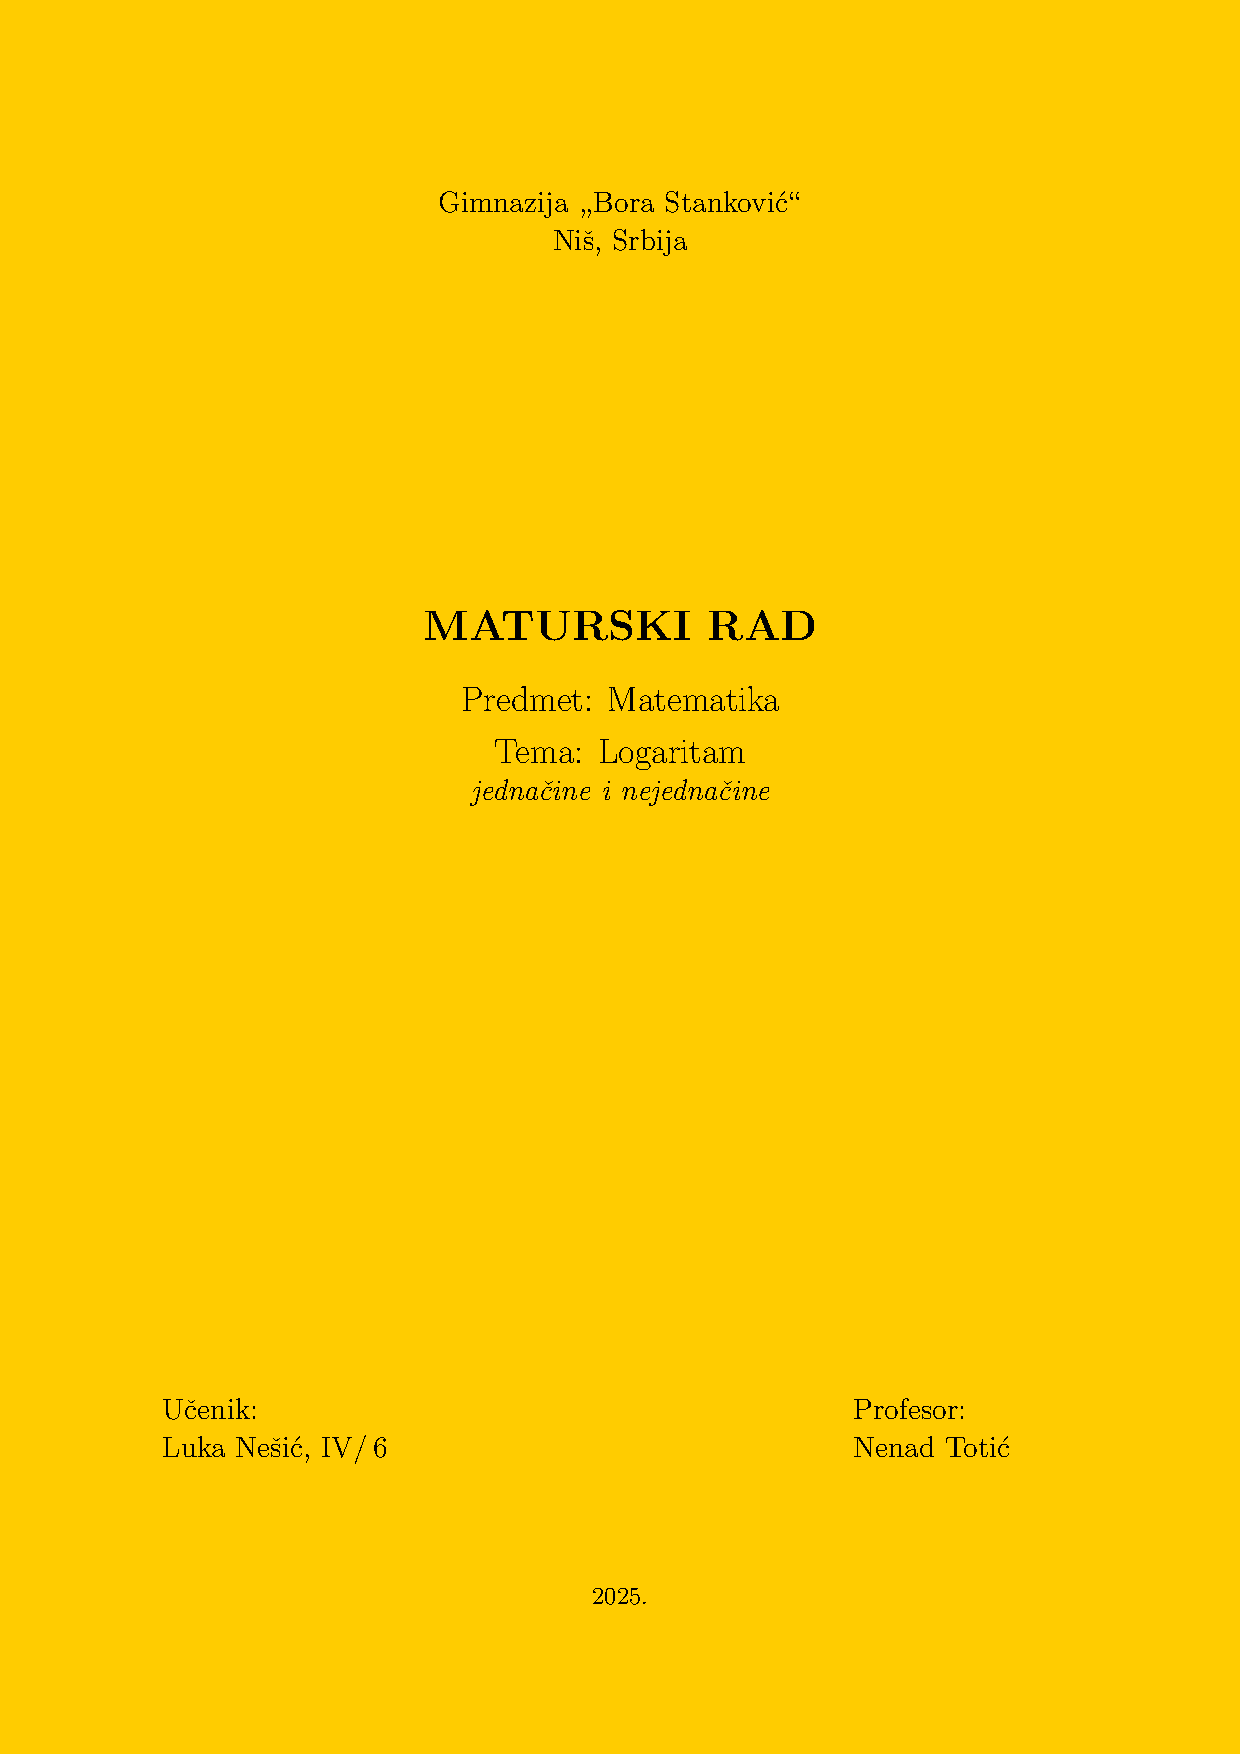
\includegraphics[]{log.5}}{Pravougli \idx{trougao}\index{pravougli trougao} $\triangle ABC$.}
$$
(Zadatak sa {Tik-Toka\index{TikTok@Tik-Tok}}.)

\resenje Na{\dj}imo najpre re{\sv}e{\nj}e op{\sv}teg slu{\cv}aja
$$
a=\ln(px),\quad b=\ln(qx),\quad c=\ln(rx).
$$
Zbog lak{\sv}eg pisa{\nj}a izvr{\sv}imo smenu% $t=\ln x$, $u=\ln p$, $v=\ln q$ i $w=\ln r$,
$$t=\ln x,\quad u=\ln p,\quad v=\ln q,\quad w=\ln r,$$
odakle je 
$$a=t+u,\quad b=t+v,\quad c=t+w.$$
Iz {\sl Pitagorine teoreme\/}\index{Pitagorina teorema} 
$a^2 + b^2 = c^2$, sledi da je
\begin{align*}
(t+u)^2 + (t+v)^2 &=(t+w)^2\\
t^2 +2tu + u^2 + t^2 + 2tv + v^2 &= t^2 + 2tw + w^2
\end{align*}
gde, nakon sre{\dj}iva{\nj}a, dobijamo kvadratnu jedna{\cv}inu\queq
$$
t^2 + 2(u+v-w)t + (u^2 + v^2 - w^2)=0,
$$
{\cv}ija su re{\sv}e{\nj}a
\begin{align*}
t_{1,2} &=
w-u-v \pm \sqrt{2(w-u)(w-v)},
\intertext{ali nas zanima samo pozitivno, odakle je, kada vratimo smenu}
\ln x &=
\ln\left(\frac{r}{p q}\right) + \sqrt{2\ln\left(\frac rp\right) \ln\left(\frac rq\right)},
\intertext{odnosno,}
x &= \frac{r}{p q}\cdot\e^{\sqrt{2\ln(r/p)\ln(r/q)}}.
\intertext{\indent Kada u ovo re{\sv}e{\nj}e stavimo vrednosti sa slike, 
$p=1$, $q=2$ i $r=3$, dobijamo da je}
x &= \ram{\frac32\, \e^{\sqrt{2\ln(3)\ln(3/2)}}}
\approx 3\.85488,
\end{align*}
a stranice trougla su pribli{\zv}no
$$
a\approx 1\.34934, \quad b\approx 2\.04249, \quad c\approx 2\.44795.
$$
(Na slici je $1=\hbox{`$\vcenter{\hbox{\rule{3truecm}{0.4truept}}}$'}$.)
